\documentclass[11pt,a4paper]{article}
\usepackage{color}
\usepackage{amsmath, amsthm, amssymb, amsfonts, verbatim}
\usepackage{graphicx}

\title{Assessing glymphatic transport velocities by adjoint methods}

\renewcommand{\comment}[1]{\textcolor{red}{#1}}

\author{Lars Magnus Valnes, Sebastian K. Mitusch, Geir A. Ringstad, Per Kristian Eide, Simon W. Funke, Kent-Andre Mardal }


\begin{document}
\maketitle

\begin{abstract}
\end{abstract}
\section{Introduction}

The discovery of the paravascular pathway in 2011~\cite{iliff2012paravascular} propose a novel component
crucial to the metabolism of the brain which may potientially provide an explanation for the accumulation of
waste such as amyloid beta in elderly, ultimately leading to diseases such as Alzheimer and Parkinson. 
In the rest of our body, the lymphatic system plays an important role
in the clearance of metabolic waste, but there are no lymphs within the brain. This fact is puzzling in particular because
the brain requires around 10 times more energy per volume than the result of the body. The paravascular 
pathway is proposed important to waste clearance and has therefore been named the \emph{glymphatic system}.      

The pioneering works of Sykov{\'a} and Nicholson~\cite{sykova2008diffusion} demonstrated
that diffusion was a governing transport mechanism in the brain. However, 
the clearance of CSF-tracers during sleep~\cite{xie2013sleep} in mice demonstrated transportation
much faster what could be explained by diffusion and it was proposed that arterial pulsation powered
accelrated perivascular flow combined convective interstitial flow. Several modelling attempts
have put the theory to the test~\cite{asgari2016glymphatic, smith2017glymphatic, holter2017interstitial}, 
but so far computational modeling have failed to adequately described the mechanism.   

Transportation by diffusion is in the order of XXX\comment{Lars: hente fra R. Thorne / Nicholson}. 
However, in \cite{xie2013sleep} a 60% coverage of 3kDa Texas Red Dextran of a $200 \mu m$ cube was demostrated in approximately 
20 minutes. As such, the transportation is XXX faster than what diffusion would provide. Furthermore, 
in \cite{eidevalnes} it was demonstrated that X Da Gadovist was brainwide in 8 hours after injection in the lumbar region.      

Paragraph about timescales etc. 

The purpose of this paper is to attempt to assess transportation speed in terms of an apparent diffusion coefficient 
by using adjoint methods provided by \cite{} for optimizing the coefficient with respect to data. As
such a coefficient larger than commonly reported values of diffusion would suggest that at the
timescale of minutes to hours there is indeed a glymphatic transportation which may potentially 
be responsible for metabolic waste.     

An outline of the paper is as follows. In Section 2 we descibe the medical images and their modality,  
and the mathematical methodology used for determining the apparent diffusion coefficients.  


\section{Methods}


\subsection*{Data}

\subsection*{Mathematical Model}
The objective function was defined as 
\begin{equation}
\min_{u,g} F = \quad \sum\limits_i\sp{n} \int\limits_{\Omega} |u(t_i) - u_{obs}(t_i)| \mathrm{d}\Omega + \frac{\alpha}{2} \int\limits_{0}\sp{T} || g ||_{L\sp{2}(\partial\Omega)} \mathrm{d}t + \frac{\beta}{2} \int\limits_{0}\sp{T} || \dot{g} ||_{L\sp{2}(\partial\Omega)}\mathrm{d}t 
\end{equation}
subjugated by   
\begin{equation}
\begin{aligned}
\frac{\partial u}{\partial t} = \nabla \cdot  D_i \nabla u \qquad \text{in} \qquad \Omega \times \left\lbrace 0 , T \right)  \\
u=g(t) \qquad \text{on} \qquad \partial\Omega  \times \left\lbrace 0 , T \right) 
\end{aligned}
\label{Eq::PDE}
\end{equation}
with the domain $\Omega$ contains three sub domains, each with a different diffusion coefficient. We denote the Cerebral Spinal fluid (CSF) domain as $\Omega_1$, the grey matter as $\Omega_2$ and the white matter as $\Omega_3$.

\section*{Manufactured Solution}
The manufactured observations was obtained by forward computation of Eq.\ref{Eq::PDE} with the Dirichlet boundary condition defined as
\begin{equation}
g(t)_{\partial \Omega_1} = 0.3 +0.167t - 0.007t\sp{2} \qquad  0 \leq t \leq 24.
\end{equation}
The timestep was $dt = 0.02$, and the diffusion coefficients were selected to be 
\begin{equation}
D_{\Omega_1} = 1000 \quad , \quad D_{\Omega_2} = 4.0 \quad , \quad D_{\Omega_3} = 8.0 
\end{equation}  
The magnitude order of the diffusion coefficient are chosen so that they resemble diffusion coefficient in csf, grey and white matter. The forward simulation gave a total of 120 possible observation time points. These points 
will be denoted as $\tau$.

The mesh was constructed by using the MRI of a patient diagnosed with iNPH. The software Freesurfer was used in segmentation and creating the polyhedral surfaces of the white and grey matter. Then the use of T2 weighted MRI was used to segment the csf compartment surrounding the cerebral. The polyhedral surfaces was used with CGAL[?] to construed the mesh. The computational requirement for the resulting mesh was significant, therefore a submesh was also constructed, see Fig. ??. 


\section*{Implementation}
The code used the FEniCS project to contruct the PDE, using backwards Euler time discretization and first order continuous galerkin finite elements. The module dolfin adjoint [?] was used to construct a reduced functional, and the optimization used the scipy optimize library to minimize the functional using L-BFGS-B algorithm.   

The implementation used the first observation as initial conditions of Eq.\ref{Eq::PDE}, and for each timestep, the next observation was used as the Dirichlet boundary conditions.  

The initial values of the optimization algorithm was chosen to be $1,1,1$. Furthermore, to obtain faster convergence in the optimization, the diffusion coefficients was scaled to have the same magnitude, i.e.  $D_{\Omega_1}$ was scaled, so that $D_{\Omega_1} = D\sp{u}_{\Omega_1}*100$.    


\section*{Non-linear relation}
The MR images are provided by Oslo University Hospital Rikshospitalet and can be seen in Fig.??. The software Freesurfer was used to segment and align each of the observations, which made it possible to estimate voxelwise intensity increase due to tracer concentrations. The tracer causes the longitudinal(spin-lattice) relaxation time $T_{1}$ to shorten with the following relation
\begin{equation}
\frac{1}{T_{1}\sp{c}} = \frac{1}{T_{1}\sp{0}} + r_{1}*C .
\label{EQ::contrast}
\end{equation}
with the superscripts indicating with contrast and without contrast and $r_1$ as the relaxivity constant for the MRI-contrast in a medium. The relation between intensity and concentration is non-linear, and is expressed with the following equations. The signal intensity $SI$ of the sequence is given by
\begin{equation}
SI = M_{n} \sin \theta e\sp{ - TE/T_2\sp{*} },
\label{EQ::SI_T2}
\end{equation}
with  $TE$ and $\theta$ respectively denoting the echo time and the flip angle. Also $T2\sp{*}$ is transverse magnetization caused by a combination of spin-spin relaxation and magnetic field inhomogeneity. It is defined as 
\begin{equation}
\frac{1}{T_2\sp{*}} = \frac{1}{T_2} + \gamma \Delta B_{in} ,
\end{equation}
with $T2$ transverse (spin-spin) relaxation time, $\gamma$ is the gyromagnetic ratio and $\Delta B_{in}$ is the magnetic field inhomogeneity
across a voxel. % We will assume that the field inhomogeneity is constant.
We will simplify the expression by neglecting the T2 term in the signal,
given that $TE <<T_2\sp{*}$ for this MRI sequence. Thus Eq. \ref{EQ::SI_T2} becomes 
\begin{equation}
SI = M_{n} \sin \theta.
\label{EQ::SI}
\end{equation}
In article [?] term $M_n$ is the magnetization in the the n-echo given as 
\begin{equation}
M_{n} = M_{0}  \left[ (1-\beta)\frac{(1-(\alpha \beta)\sp{n-1} }{1-\alpha\beta} + (\alpha \beta)\sp{n-1}(1-\gamma) + \gamma ( \alpha \beta)\sp{n-1} \frac{M_{e}}{M_{0}}  \right]   
\end{equation}
with 
\begin{equation}
\frac{M_{e}}{M_{0}} = - \left[ \frac{ 1 -\delta + \alpha \delta (1-\beta ) \frac{1-\alpha\beta\sp{m}}{1-\alpha \beta} + \alpha\delta(\alpha\beta)\sp{m-1} - \alpha\sp{m}\rho}{1 +\rho \alpha\sp{m} } \right].
\end{equation}
Using the following definitions
\begin{equation}
\begin{aligned}
\alpha &= \cos ( \theta ) \\
\beta  &= e\sp{- \sp{T_b}/_{T_1}\sp{0} } \\
\delta &= e\sp{- \sp{T_a}/_{T_1}\sp{0} } \\
\gamma &= e\sp{- \sp{T_w}/_{T_1}\sp{0} } \\
\rho   &= e\sp{- \sp{TR}/_{T_1}\sp{0} }  \\
T_w    &= TR - T_a -T_b(m-1)       .\\
\end{aligned}
\end{equation}
Here $T_b$ is known as the echo spacing, $T_a$ is the inversion time, $T_w$ the time delay, $TR$ as the repetition time, $m$ is the number of echo spacings and $T1$ is the longitudinal(spin-lattice) relaxation time for a given medium. The $M_0$ is a calibration constant of the magnetization. The center echo denoted as $n=\sp{m}/_2$ will be the signal that we will consider when estimating MRI-contrast.



 

\begin{itemize}
\item describe the imaging, shortly with ref to JCI  
\item describe the abstract mathematical problem to be solved, ie. PDE constrained opt problem where we 
address coefficients and bc  
\item the details: finite element, reduced problem, BFGS,  
\end{itemize}

\begin{figure}
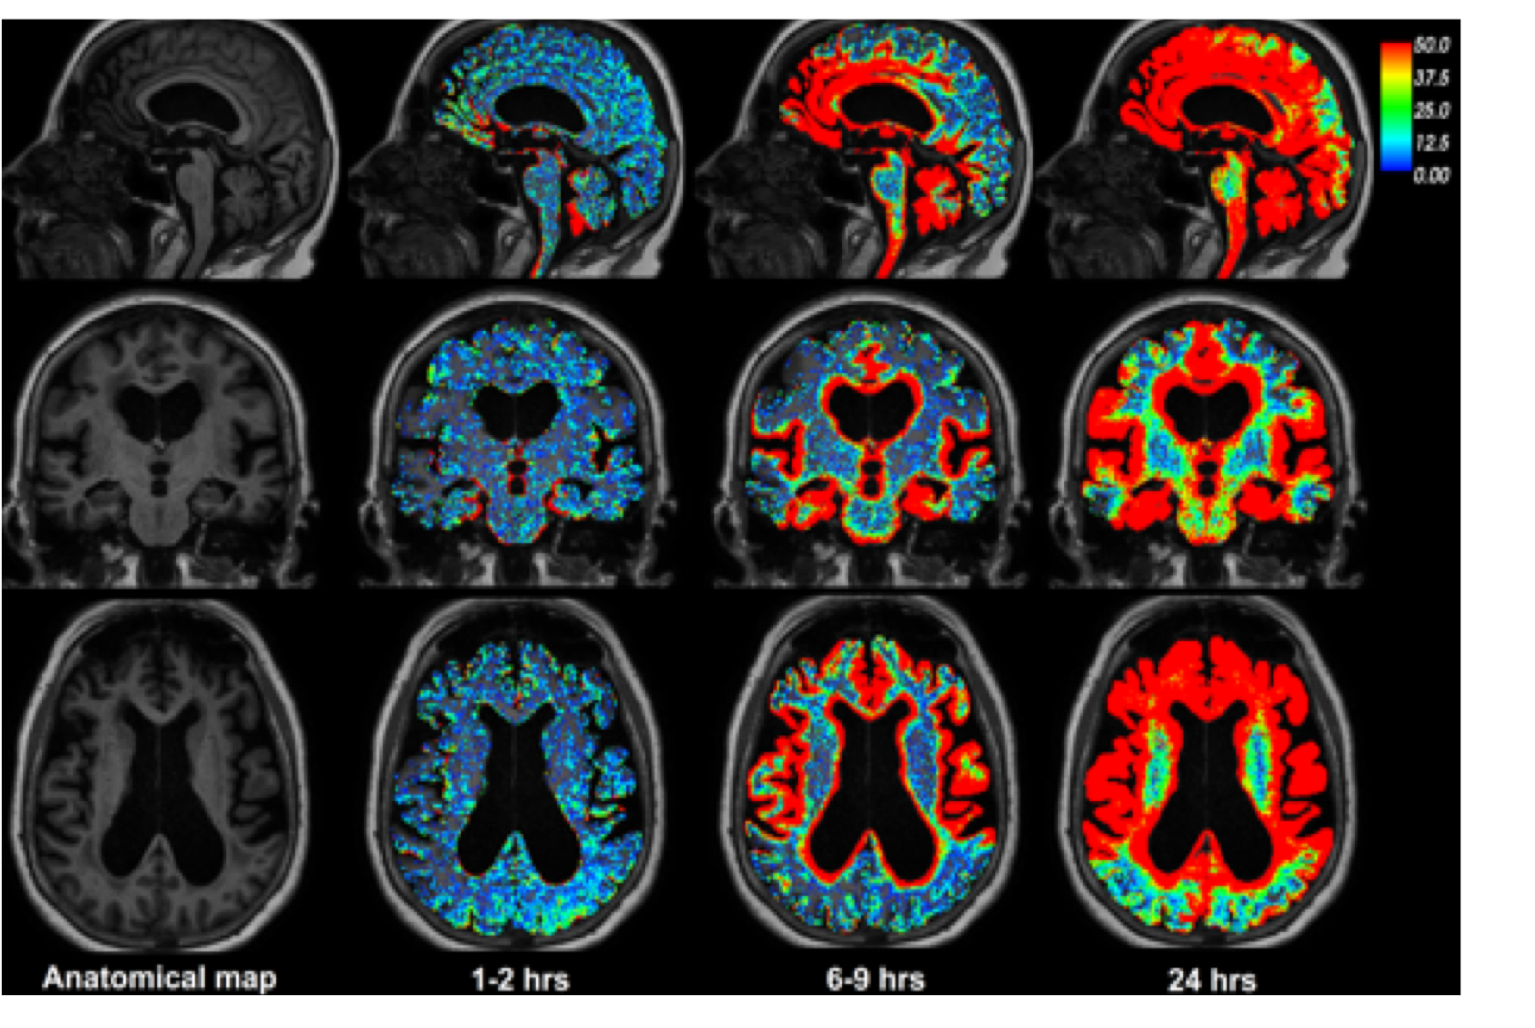
\includegraphics[width=0.95\textwidth]{GMRI.png} 
\label{fig1} 
\caption{\comment{lars, we will need some new images since I believe this is stolen from JCI}}
\end{figure}

\comment{Lars: bilde av konkret mesh  }

\begin{figure}
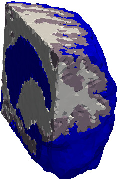
\includegraphics[width=0.3\textwidth]{mesh-eps-converted-to.pdf} 
\label{fig1} 
\caption{\comment{lars, we will need some new images since I believe this is stolen from JCI}}
\end{figure}


\section{Results}
\begin{itemize}
\item 2D experiments as have already been done (with and without noise/ with and without observations everywhere in time) 
\item 2D experiments should highlight the impact of the regularization parameter wrt number of iterations and diffusion 
coeff 
\item 3D experiments based on data generated  
\item 3D experiments based on real data (\comment{lars: we need to try testing this}) 
\end{itemize}



The results.

The optimal relaxation parameters was investigated by using 10 evenly spaced time points as observations. Then estimate the corresponding controls, while varying the relaxation parameters.


The dependency on the spacing and distribution of $tau$ was done by using the optimal relaxation parameters and consider number of time points equal to the number of observations. 


The dependency of time steps were computed by increasing the times



The dependency on noise was done by adding randomly distributed noise to the observations.

There are some extreme cases that require some considerations, namely :

no observations around 12, i.e. can the parameters be estimated if there exists a hole in the observations.

Is estimating parameters between 2























\begin{table}
\centering
\caption{Shows the relaxation parameters $\alpha$ and $\beta$, number of timesteps $k$ and number of observation $\tau$ with the resulting number of iterations and estimated optimal parameters for the diffusion coefficients. }
\resizebox{\textwidth}{!}{\begin{tabular}{*{8}c}
$\alpha$ & $\beta$ & k & $\tau$ & iter & $ D_{\Omega_1} = 1000$ & $ D_{\Omega_2} = 4.0 $ & $D_{\Omega_3} = 8.0 $ \\
\hline
 1.0 & 1.0 &10 &10 & 801& 3152.55150305 & 5.66843317507 & 9.10176601537 \\
 1.0 & 0.1 &10 &10 & 846& 2890.10652122 & 5.8333990243 & 9.14516904881   \\
 1.0 & 0.01 &10 &10 & 1001& 2374.75510786 & 5.90748588887 & 9.1624514977  \\ 
 1.0 & 0.001 &10 &10 & 987& 3012.94145621 & 5.84828588848 & 9.14780994071 \\
 1.0 & 0.0001 &10 &10 & 1001& 2846.67368004 & 5.86716070687 & 9.1516059019 \\
 1.0 & 1e-05 &10 &10 & 1001& 2488.99687704 & 5.89553108585 & 9.16094907807 \\
 1.0 & 1e-06 &10 &10 & 1001& 2572.74685463 & 5.88550285289 & 9.15701445733 \\
 0.1 & 1.0 &10 &10 & 525& 1165.00025805 & 4.55541673123 & 8.51469574502 \\
 0.1 & 0.1 &10 &10 & 899& 1098.5603179 & 4.5965351918 & 8.60353462124 \\
 0.1 & 0.01 &10 &10 & 792& 1148.68286947 & 4.58961131725 & 8.60923608344 \\ 
 0.1 & 0.001 &10 &10 & 768& 1133.11485657 & 4.59512891707 & 8.61427396989 \\
 0.1 & 0.0001 &10 &10 & 840& 1152.61459776 & 4.5895138786 & 8.61107565287 \\
 0.1 & 1e-05 &10 &10 & 739& 1145.12699776 & 4.59168203791 & 8.61245925367 \\
 0.1 & 1e-06 &10 &10 & 697& 1127.51137739 & 4.59724924241 & 8.6163255093 \\
 0.01 & 1.0 &10 &10 & 130& 1000.69417631 & 4.45194182806 & 8.48016213899 \\
 0.01 & 0.1 &10 &10 & 204& 1001.45906364 & 4.44288397852 & 8.55964437402 \\
 0.01 & 0.01 &10 &10 & 384& 1004.91771072 & 4.44039285507 & 8.57773362809 \\
 0.01 & 0.001 &10 &10 & 455& 1006.92821746 & 4.4401364227 & 8.57964644068 \\
 0.01 & 0.0001 &10 &10 & 382& 1005.46132856 & 4.44059403278 & 8.58161935877 \\
 0.01 & 1e-05 &10 &10 & 389& 1005.48872458 & 4.44091328174 & 8.58070451064 \\
 0.01 & 1e-06 &10 &10 & 320& 1003.88180045 & 4.44140148563 & 8.57914151398 \\
 0.001 & 1.0 &10 &10 & 144& 1000.72690068 & 4.43617090765 & 8.47356658247 \\
 0.001 & 0.1 &10 &10 & 188& 1001.11632883 & 4.42560354452 & 8.55339645884 \\
 0.001 & 0.01 &10 &10 & 242& 1002.06937059 & 4.42388003439 & 8.57511846108 \\
 0.001 & 0.001 &10 &10 & 332& 1005.24945351 & 4.42278572482 & 8.58013052115 \\
 0.001 & 0.0001 &10 &10 & 432& 1008.05660576 & 4.42186842634 & 8.58305135552 \\
 0.001 & 1e-05 &10 &10 & 360& 1006.05061062 & 4.42295196846 & 8.57964172911 \\
 0.001 & 1e-06 &10 &10 & 363& 1006.70468432 & 4.42251369108 & 8.58151348789 \\
 0.0001 & 1.0 &10 &10 & 157& 1000.83218743 & 4.43452507573 & 8.47318916943 \\
 0.0001 & 0.1 &10 &10 & 131& 1000.56624899 & 4.42351929725 & 8.55256760219 \\
 0.0001 & 0.01 &10 &10 & 174& 1001.0091989 & 4.42260942583 & 8.57478259945 \\
 0.0001 & 0.001 &10 &10 & 136& 1000.57577092 & 4.4239534819 & 8.57151355191 \\
 0.0001 & 0.0001 &10 &10 & 283& 1003.03255695 & 4.42248562737 & 8.5786695754 \\
 0.0001 & 1e-05 &10 &10 & 284& 1003.54402535 & 4.42227734882 & 8.58311915306 \\
 0.0001 & 1e-06 &10 &10 & 289& 1003.03642353 & 4.42224580212 & 8.58006825258 \\
 1e-05 & 1.0 &10 &10 & 151& 1000.79310038 & 4.43448500449 & 8.47338153139 \\
 1e-05 & 0.1 &10 &10 & 140& 1000.70858373 & 4.42340629909 & 8.55312689863 \\
 1e-05 & 0.01 &10 &10 & 203& 1001.34714912 & 4.42253540005 & 8.57470943099 \\
 1e-05 & 0.001 &10 &10 & 215& 1001.75591211 & 4.42292580709 & 8.58079455564 \\
 1e-05 & 0.0001 &10 &10 & 208& 1001.41103854 & 4.42264942624 & 8.58064686718 \\
 1e-05 & 1e-05 &10 &10 & 218& 1001.73103534 & 4.42318548221 & 8.57843152546 \\
 1e-05 & 1e-06 &10 &10 & 191& 1001.33680306 & 4.42244263068 & 8.58128891831 \\
 1e-06 & 1.0 &10 &10 & 115& 1000.47868283 & 4.43456295486 & 8.47226911091 \\
 1e-06 & 0.1 &10 &10 & 158& 1000.8203239 & 4.42368702618 & 8.55236552474 \\
 1e-06 & 0.01 &10 &10 & 142& 1000.64224198 & 4.42327990324 & 8.57047799569 \\
 1e-06 & 0.001 &10 &10 & 149& 1000.64956243 & 4.42317461499 & 8.57554522252 \\
 1e-06 & 0.0001 &10 &10 & 179& 1001.07075407 & 4.42262619987 & 8.57788936678 \\
 1e-06 & 1e-05 &10 &10 & 254& 1002.49656481 & 4.42254606227 & 8.58162265954 \\
 1e-06 & 1e-06 &10 &10 & 228& 1001.78781526 & 4.42297193581 & 8.57946804203 \\
\end{tabular}}
\label{Tab::1}
\end{table} 


\begin{table}
\centering
\caption{ }
\resizebox{\textwidth}{!}{\begin{tabular}{*{8}c}
$\alpha$ & $\beta$ & k & $\tau$ & iter & $ D_{\Omega_1} = 1000$ & $ D_{\Omega_2} = 4.0 $ & $D_{\Omega_3} = 8.0 $ \\
\hline
 0.1 & 1.0 &40 &10 & 743& 1187.4771691 & 4.35026181483 & 8.09946730636 \\ 
 0.1 & 0.1 &40 &10 & 932& 1555.16869771 & 6.09495269829 & 8.50884374613 \\ 
 0.1 & 0.01 &40 &10 & 1001& 3568.28083904 & 29.3015755902 & 44.1578313645 \\ 
 0.1 & 0.001 &40 &10 & 1001& 3910.1049326 & 35.4922989536 & 56.545598289 \\ 
 0.1 & 0.0001 &40 &10 & 1001& 4628.35215443 & 39.7391559549 & 63.5747349342 \\ 
 0.1 & 1e-05 &40 &10 & 1001& 4402.68260002 & 38.7772764366 & 62.3107416526 \\ 
 0.1 & 1e-06 &40 &10 & 1001& 4048.23822112 & 36.8496309935 & 58.8659971438 \\ 
 0.01 & 1.0 &40 &10 & 291& 1000.67788636 & 4.02002908826 & 7.98566981348 \\ 
 0.01 & 0.1 &40 &10 & 185& 1000.41583989 & 4.15725853533 & 8.04068211749 \\ 
 0.01 & 0.01 &40 &10 & 770& 1010.05721903 & 4.46873471103 & 8.23345999428 \\ 
 0.01 & 0.001 &40 &10 & 906& 1035.3816137 & 5.23577439946 & 8.93787811692 \\ 
 0.01 & 0.0001 &40 &10 & 933& 1054.26269562 & 5.75801399377 & 9.64500568339 \\ 
 0.01 & 1e-05 &40 &10 & 816& 1047.05756594 & 5.84828880596 & 9.82387355658 \\ 
 0.01 & 1e-06 &40 &10 & 788& 1040.16446365 & 5.75691158325 & 9.6813276929 \\ 
 0.001 & 1.0 &40 &10 & 221& 1000.18451793 & 3.98737893359 & 7.97554944332 \\ 
 0.001 & 0.1 &40 &10 & 330& 1000.32828904 & 4.04755624182 & 8.0244839499 \\ 
 0.001 & 0.01 &40 &10 & 362& 1000.3803523 & 4.11154445121 & 8.11157880655 \\ 
 0.001 & 0.001 &40 &10 & 657& 1001.71334392 & 4.19267152271 & 8.27191901359 \\ 
 0.001 & 0.0001 &40 &10 & 1001& 1004.86321852 & 4.26170953011 & 8.44356313497 \\ 
 0.001 & 1e-05 &40 &10 & 815& 1004.02931722 & 4.37346057066 & 8.57873677626 \\ 
 0.001 & 1e-06 &40 &10 & 802& 1004.22491712 & 4.37575380922 & 8.58549567766 \\ 
 0.0001 & 1.0 &40 &10 & 172& 1000.08077115 & 3.98137276814 & 7.97389541303 \\ 
 0.0001 & 0.1 &40 &10 & 284& 1000.13089398 & 4.03045319152 & 8.02261617711 \\ 
 0.0001 & 0.01 &40 &10 & 330& 1000.10285205 & 4.08364875893 & 8.09505305597 \\ 
 0.0001 & 0.001 &40 &10 & 559& 1000.5278853 & 4.10885628451 & 8.19383426091 \\ 
 0.0001 & 0.0001 &40 &10 & 342& 1000.14882303 & 4.11658048605 & 8.17742760473 \\ 
 0.0001 & 1e-05 &40 &10 & 321& 1000.08672575 & 4.05337754766 & 8.14081741343 \\ 
 0.0001 & 1e-06 &40 &10 & 551& 1000.58380151 & 4.09044639474 & 8.25619973521 \\ 
 1e-05 & 1.0 &40 &10 & 173& 1000.08653936 & 3.98154190918 & 7.97388822692 \\ 
 1e-05 & 0.1 &40 &10 & 343& 1000.20326692 & 4.03035382968 & 8.02271998911 \\ 
 1e-05 & 0.01 &40 &10 & 419& 1000.31305287 & 4.07478958493 & 8.10307012855 \\ 
 1e-05 & 0.001 &40 &10 & 437& 1000.2320762 & 4.08452785122 & 8.16938871213 \\ 
 1e-05 & 0.0001 &40 &10 & 374& 1000.11697131 & 4.07952084401 & 8.15715261877 \\ 
 1e-05 & 1e-05 &40 &10 & 463& 1000.29010188 & 4.08615998822 & 8.20191735247 \\ 
 1e-05 & 1e-06 &40 &10 & 624& 1000.69464905 & 4.08563263518 & 8.25675573539 \\ 
 1e-06 & 1.0 &40 &10 & 232& 1000.18034176 & 3.98264060176 & 7.97405892351 \\ 
 1e-06 & 0.1 &40 &10 & 287& 1000.15080505 & 4.02963675823 & 8.02269997607 \\ 
 1e-06 & 0.01 &40 &10 & 403& 1000.24828839 & 4.07422258869 & 8.09935561335 \\ 
 1e-06 & 0.001 &40 &10 & 363& 1000.16258199 & 4.10092887055 & 8.17481714787 \\ 
 1e-06 & 0.0001 &40 &10 & 413& 1000.21453049 & 4.09366239057 & 8.19045283723 \\ 
 1e-06 & 1e-05 &40 &10 & 474& 1000.34636737 & 4.09817444633 & 8.22081707472 \\ 
 1e-06 & 1e-06 &40 &10 & 475& 1000.33096416 & 4.0786358152 & 8.20801753144 \\ 
\end{tabular}}
\label{Tab::1}
\end{table} 





\begin{table}
\centering
\caption{ $\tau = [1.0, 1.2, 1.4, 2.8, 4.6, 9.6, 14.4, 18.6, 22.2, 24.0] $}
\resizebox{\textwidth}{!}{\begin{tabular}{*{7}c}
$\alpha$ & $\beta$ & k & iter & $ D_{\Omega_1} = 1000$ & $ D_{\Omega_2} = 4.0 $ & $D_{\Omega_3} = 8.0 $ \\
\hline
 0.0001 & 1.0  &20 & 352& 1005.22142783 & 3.82672281427 & 7.96012835843 \\ 
 0.0001 & 0.1  &20 & 424& 1000.74372847 & 3.48769752552 & 7.46363505824 \\ 
 0.0001 & 0.01 &20 & 709& 996.472422218 & 3.28651606815 & 6.89922591307 \\ 
 1e-05 & 1.0   &20 & 359& 1005.8332351 & 3.82683123783 & 7.96093977635 \\ 
 1e-05 & 0.1   &20 & 413& 1000.71223403 & 3.48709269446 & 7.46388730417 \\ 
 1e-05 & 0.01  &20 & 866& 995.496494833 & 3.28703772862 & 6.89839201709 \\ 
 1e-06 & 1.0   &20 & 330& 1005.36588332 & 3.82652618763 & 7.95958068842 \\ 
 1e-06 & 0.1   &20 & 390& 1000.66722857 & 3.48707900673 & 7.46307424723 \\ 
 1e-06 & 0.01  &20 & 577& 997.407662104 & 3.28668627585 & 6.90093340281 \\ 
 0.0001 & 1.0  &40 & 720& 1144.48441614 & 4.11378216282 & 8.06601345536 \\ 
 0.0001 & 0.1  &40 & 275& 1002.81529271 & 4.01476313602 & 7.99370457785 \\ 
 0.0001 & 0.01 &40 & 309& 1003.01379879 & 3.89792451751 & 7.84348036932 \\ 
 1e-05 & 1.0   &40 & 574& 1114.40281674 & 4.11652975001 & 8.06793246669 \\ 
 1e-05 & 0.1   &40 & 402& 1005.8301423 & 4.01204511666 & 7.98950535021 \\ 
 1e-05 & 0.01  &40 & 415& 1005.8339426 & 3.89483734096 & 7.83476748243 \\ 
 1e-06 & 1.0   &40 & 648& 1124.35106201 & 4.1148536647 & 8.06730484009 \\ 
 1e-06 & 0.1   &40 & 324& 1004.23408094 & 4.01236138465 & 7.99051228829 \\ 
 1e-06 & 0.01  &40 & 444& 1007.3125095 & 3.89431330176 & 7.83169391549 \\ 
\end{tabular}}
\label{Tab::1}
\end{table} 
\section{Discussion}


\begin{table}
\centering
\caption{ $\tau =[1.2, 1.4, 1.8, 2.4, 3.6, 5.4, 7.6, 17.2, 18.6, 20.4, 22.4, 24.0] $}
\resizebox{\textwidth}{!}{\begin{tabular}{*{7}c}
$\alpha$ & $\beta$ & k & iter & $ D_{\Omega_1} = 1000$ & $ D_{\Omega_2} = 4.0 $ & $D_{\Omega_3} = 8.0 $ \\
\hline
 0.0001 & 1.0 &40 &  423& 1016.53589451 & 4.09744503422 & 8.10477831272 \\ 
 0.0001 & 0.1 &40 & 256& 1002.72187136 & 4.01772473372 & 8.01115341448 \\ 
 0.0001 & 0.01 &40& 255& 1001.77895566 & 3.940658633 & 7.89664871352 \\ 
 1e-05 & 1.0 &40  & 390& 1011.67921461 & 4.09786927743 & 8.10526579439 \\ 
 1e-05 & 0.1 &40  & 225& 1001.94506087 & 4.01805587572 & 8.01180925344 \\ 
 1e-05 & 0.01 &40 & 209& 1001.27411467 & 3.94131058751 & 7.90365080657 \\ 
 1e-06 & 1.0 &40  & 413& 1017.04677284 & 4.097319886 & 8.10398937661 \\ 
 1e-06 & 0.1 &40  & 240& 1002.43313972 & 4.01777944191 & 8.01163086184 \\ 
 1e-06 & 0.01 &40 & 356& 1003.33076616 & 3.93893764944 & 7.88611881889 \\ 
\end{tabular}}
\label{Tab::1}
\end{table} 
\section{Discussion}


 \begin{table}
\centering
\caption{ $\tau = [2.4, 4.8, 7.2, 9.6, 12.0, 14.4, 16.8, 19.2, 21.6, 24.0] $}
\resizebox{\textwidth}{!}{\begin{tabular}{*{7}c}
$\alpha$ & $\beta$ & k & iter & $ D_{\Omega_1} = 1000$ & $ D_{\Omega_2} = 4.0 $ & $D_{\Omega_3} = 8.0 $ \\
\hline
 0.001 & 1.0 &11   & 535& 1155.41620776 & 4.56890164554 & 8.74862316292 \\ 
 0.001 & 0.1 &11  & 692& 1138.18797804 & 4.77615608916 & 9.1001502642 \\ 
 0.001 & 0.01 &11 & 620& 1109.09332378 & 4.83440528908 & 9.23937192655 \\ 
 0.0001 & 1.0 &11 & 512& 1177.95965037 & 4.56118986925 & 8.74503026051 \\ 
 0.0001 & 0.1 &11 & 796& 1167.15728007 & 4.76942041977 & 9.09708917746 \\ 
 0.0001 & 0.01&11 & 726& 1147.45125238 & 4.82397769456 & 9.23132854631 \\ 
 1e-05 & 1.0 &11  & 547& 1150.09091484 & 4.56745099896 & 8.74784724393 \\ 
 1e-05 & 0.1 &11  & 774& 1209.27556281 & 4.7599962838 & 9.09240730332 \\ 
 1e-05 & 0.01 &11 & 963& 1178.62113472 & 4.81968561039 & 9.22165857548 \\ 
 1e-06 & 1.0 &11  & 516& 1178.30282045 & 4.56182347972 & 8.74408755566 \\ 
 1e-06 & 0.1 &11  & 690& 1169.85258682 & 4.76763208109 & 9.09437803203 \\ 
 1e-06 & 0.01 &11 & 885& 1161.54226173 & 4.82290410594 & 9.23253559953 \\ 
 0.001 & 1.0 &10  & 144& 1000.72690068 & 4.43617090765 & 8.47356658247 \\ 
 0.001 & 0.1 &10  & 188& 1001.11632883 & 4.42560354452 & 8.55339645884 \\ 
 0.001 & 0.01 &10 & 242& 1002.06937059 & 4.42388003439 & 8.57511846108 \\ 
 0.0001 & 1.0 &10 & 157& 1000.83218743 & 4.43452507573 & 8.47318916943 \\ 
 0.0001 & 0.1 &10 & 131& 1000.56624899 & 4.42351929725 & 8.55256760219 \\ 
 0.0001 & 0.01&10 & 174& 1001.0091989 & 4.42260942583 & 8.57478259945 \\ 
 1e-05 & 1.0 &10  & 151& 1000.79310038 & 4.43448500449 & 8.47338153139 \\ 
 1e-05 & 0.1 &10  & 140& 1000.70858373 & 4.42340629909 & 8.55312689863 \\ 
 1e-05 & 0.01 &10 & 203& 1001.34714912 & 4.42253540005 & 8.57470943099 \\ 
 1e-06 & 1.0 &10  & 115& 1000.47868283 & 4.43456295486 & 8.47226911091 \\ 
 1e-06 & 0.1 &10  & 158& 1000.8203239 & 4.42368702618 & 8.55236552474 \\ 
 1e-06 & 0.01 &10 & 142& 1000.64224198 & 4.42327990324 & 8.57047799569 \\ 
 0.001 & 1.0 &10  & 127& 1000.57534928 & 4.43620469807 & 8.47334881884 \\ 
 0.001 & 0.1 &10  & 209& 1001.40602027 & 4.42496040369 & 8.55523771434 \\ 
 0.001 & 0.01 &10 & 212& 1001.64339174 & 4.42433050528 & 8.57315746956 \\ 
 0.0001 & 1.0 &9  & 110& 999.72163906 & 4.11479310934 & 8.33462232991 \\ 
 0.0001 & 0.1 &9  & 105& 999.69280754 & 4.1045396919 & 8.33774014666 \\ 
 0.0001 & 0.01 &9 &  88& 999.772427775 & 4.10360542672 & 8.33814068545 \\ 
 1e-05 & 1.0 &9   & 129& 999.64486142 & 4.11473526399 & 8.33422818516 \\ 
 1e-05 & 0.1 &9   & 127& 999.585578036 & 4.10455462113 & 8.3375263256 \\ 
 1e-05 & 0.01 &9  &  91& 999.743943666 & 4.10325272534 & 8.33837761724 \\ 
 1e-06 & 1.0 &9   & 138& 999.565361602 & 4.11477304552 & 8.3344417303 \\ 
 1e-06 & 0.1 &9   & 127& 999.556729496 & 4.10443164325 & 8.33788684648 \\ 
 1e-06 & 0.01 &9  & 142& 999.44777782 & 4.10347962986 & 8.33800635508 \\ 
\end{tabular}}
\label{Tab::Incoherence}
\end{table} 
\section{Discussion}

The timestep incoherence between observations and Eq.\ref{Eq::PDE} was not initially considered, since the actual data do not maintain a constant timestep of the observations. However, due to the implementation this effect became apparent when the number of timesteps changed. In Tab.\ref{Tab::Incoherence} we can see that changing the number of timesteps with 1 can improve or worsen the process significantly, both parameter estimation and number of iterations. This effect mainly comes from the proximity of the observation timepoint it is.  Therefore selecting more number of timesteps than observation points seems proficient. However, using adaptive timestepping can provide means to decrease the number of iterations, but would require 




 
The Eq.\ref{Eq::PDE} was discretized using first order Euler, thus the approximation  




We can see in Fig.??, that increasing the number of timesteps will improve the estimation of diffusion coefficients. 


The manufactured observations were constructed by imposing a quadratic function ?? as Dirichlet boundary conditions. Thus the number of time steps will affect the approximation of the boundary conditions


Thus 

The L-BFGS-B algorithm does not scale the control parameters, thus the step size . This poses a problem with a large difference in the control parameters, 




In Fig.??, we let the 
The addition of scaling the parameter $D_{\Omega_1}$ was done, such that all the diffusion parameters were in the same order of magnitude.   



There is a need for observable change in order to estimate the parameters. But considering the magnitude difference between diffusion coefficients. It is clear that the observable change is in different timescales. This prompted that in using actual data, we will only consider a mesh with 2 subdomains that have diffusion coefficient of similar magnitude.   



The case of an observation vacancy did not show any clear discrepancy in the objective function, see Fig. ??. However, there is a divergent tendency in the estimation of $D_{\Omega_1}$, see Fig.??. This same tendency can be seen in Fig. ?? with . Although this behavior  ... 


The corresponding objective function does not exhibit any discrepancy, thus the object functions dependency on $D_{\Omega_1}$ is small. 

Or rather the observation function does not compute a difference. The observation function require that the parameters presence in the observations are distinct. This is not the case for cube that reach equilibrium after one timestep. 

The mesh cells are of the order $\mathrm{mm}$ and the timesteps are of order $0.1$. The number of cells representing the csf is 15000.    
  




\bibliographystyle{amsplain}
\bibliography{references}


\end{document}


